\begin{figure}
	\centering
	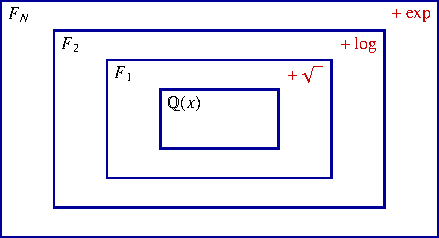
\includegraphics[width=0.7\textwidth]{papers/elliptisch/images/koerperturm.pdf}
	\caption{Eine elementare Funktion liegt in einem endlichen Turm
	von Körpererweiterungen, ausgehend von den rationalen Funktionen
	$\mathbb{Q}(x)$.
	In jedem Schritt kommt eine Wurzel, ein Logarithmus oder eine
	Exponentialfunktion dazu.}
	\label{fig:elliptisch:koerperturm}
\end{figure}
